%==============================================================================
%  BAB III - PENGUJIAN
%==============================================================================
\section{Pengujian}

Bagian ini menyajikan enam kasus uji unik yang mencakup penugasan, ekspresi
aritmatika dan relasional, ekspresi bersarang, alur kontrol, serta dua kasus
penanganan error runtime. Setiap kasus menampilkan kode sumber Arion sebagai
masukan, Intermediate Code yang dihasilkan, dan keluaran nyata program. Seluruh
hasil di bawah diperoleh dengan menjalankan kompiler pada berkas uji yang
bersangkutan; bukti tangkapan layar disertakan sebagai placeholder.

%------------------------------------------------------------------------------
\subsection{Kasus 1 -- Penugasan dan Cetak Literal}

\textbf{Tujuan.} Memverifikasi alokasi memori (\texttt{INT}), penugasan literal ke
variabel (\texttt{LIT}+\texttt{STO}), pembacaan kembali (\texttt{LOD}), dan
penimpaan nilai variabel.

\begin{minipage}[t]{0.48\textwidth}
\textbf{Masukan} (\texttt{src\_assignment.txt}):
\begin{lstlisting}[style=kodeArion, numbers=none]
program SimpleAssign;
var
  n: integer;
begin
  n := 10;
  writeln(n);
  n := 99;
  writeln(n);
end.
\end{lstlisting}
\end{minipage}\hfill
\begin{minipage}[t]{0.48\textwidth}
\textbf{Intermediate Code:}
\begin{lstlisting}[style=kodeTAC, numbers=none]
1 INT 0 4
2 LIT 0 10
3 STO 0 3
4 LOD 0 3
5 OPR 0 14
6 LIT 0 99
7 STO 0 3
8 LOD 0 3
9 OPR 0 14
10 RET 0 0
\end{lstlisting}
\end{minipage}

\textbf{Keluaran Program:}
\begin{lstlisting}[style=kodeTAC, numbers=none]
10
99
\end{lstlisting}

\begin{center}
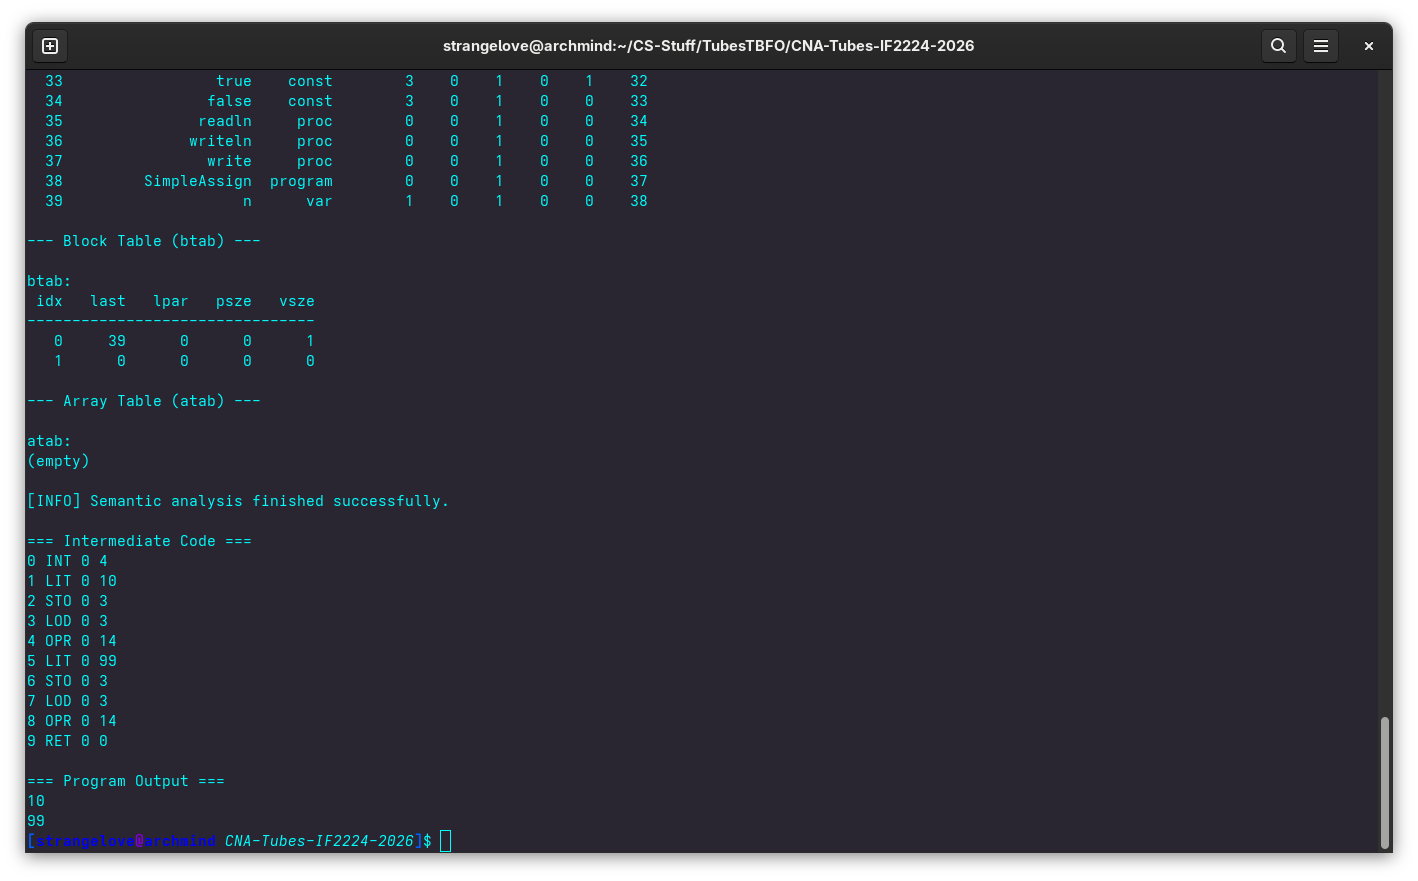
\includegraphics[width=14cm]{gambar/tc1_src_assignment.png}
\end{center}

\textbf{Analisis.} Variabel \texttt{n} dipetakan ke alamat 3 sehingga \texttt{INT}
mengalokasikan 4 sel (3 administratif + 1 variabel). Penimpaan \texttt{n := 99}
menyimpan ulang ke alamat yang sama. Keluaran sesuai harapan.

%------------------------------------------------------------------------------
\subsection{Kasus 2 -- Ekspresi Aritmatika dan Relasional}

\textbf{Tujuan.} Menguji operator aritmatika (\texttt{+}, \texttt{-}, \texttt{*},
\texttt{div}), prioritas tanda kurung, serta operator relasional yang menghasilkan
nilai \texttt{boolean}.

\begin{minipage}[t]{0.48\textwidth}
\textbf{Masukan} (\texttt{src\_expr\_assign.txt}):
\begin{lstlisting}[style=kodeArion, numbers=none]
program ExprAssign;
var
  a, b, c: integer;
begin
  a := 6 + 4;
  b := (a - 2) * 3;
  c := b div 5;
  writeln(a);
  writeln(b);
  writeln(c);
  writeln(a = 10);
  writeln(b > c);
end.
\end{lstlisting}
\end{minipage}\hfill
\begin{minipage}[t]{0.48\textwidth}
\textbf{Intermediate Code:}
\begin{lstlisting}[style=kodeTAC, numbers=none]
1 INT 0 6      16 LOD 0 3
2 LIT 0 6      17 OPR 0 14
3 LIT 0 4      18 LOD 0 4
4 OPR 0 2      19 OPR 0 14
5 STO 0 3      20 LOD 0 5
6 LOD 0 3      21 OPR 0 14
7 LIT 0 2      22 LOD 0 3
8 OPR 0 3      23 LIT 0 10
9 LIT 0 3      24 OPR 0 7
10 OPR 0 4     25 OPR 0 14
11 STO 0 4     26 LOD 0 4
12 LOD 0 4     27 LOD 0 5
13 LIT 0 5     28 OPR 0 11
14 OPR 0 5     29 OPR 0 14
15 STO 0 5     30 RET 0 0
\end{lstlisting}
\end{minipage}

\textbf{Keluaran Program:}
\begin{lstlisting}[style=kodeTAC, numbers=none]
10
24
4
TRUE
TRUE
\end{lstlisting}

\begin{center}
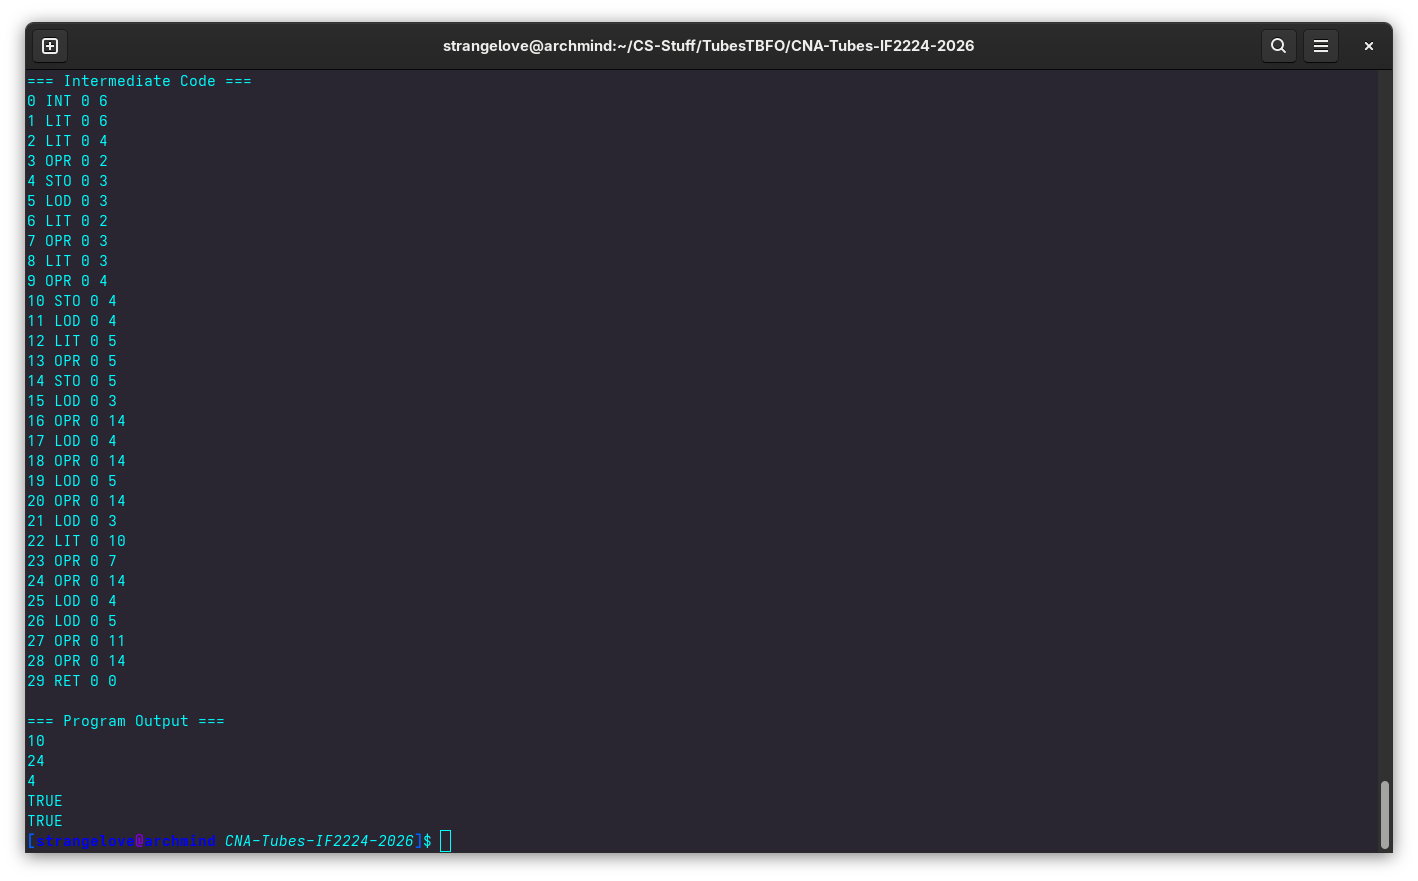
\includegraphics[width=15cm]{gambar/tc2_src_expr_assign.png}
\end{center}

\textbf{Analisis.} Perhitungan terverifikasi: $a = 10$, $b = (10-2)\times 3 = 24$,
$c = 24 \div 5 = 4$ (pembagian integer). Operator relasional \texttt{=} (OPR 7) dan
\texttt{>} (OPR 11) menghasilkan \texttt{boolean} yang dicetak sebagai
\texttt{TRUE}.

%------------------------------------------------------------------------------
\subsection{Kasus 3 -- Ekspresi Bersarang dan Modulus}

\textbf{Tujuan.} Memastikan penelusuran DFS meratakan ekspresi bersarang
\texttt{(a + b) * (c - d)} dengan benar---hasil antara ditinggalkan di puncak
stack sebagai pengganti variabel sementara---serta menguji operator \texttt{mod}.

\begin{minipage}[t]{0.48\textwidth}
\textbf{Masukan} (\texttt{src\_nested\_expr.txt}):
\begin{lstlisting}[style=kodeArion, numbers=none]
program NestedExpr;
var
  a, b, c, d, x: integer;
begin
  a := 3;  b := 4;
  c := 10; d := 2;
  x := (a + b) * (c - d);
  writeln(x);
  writeln(c mod d);
end.
\end{lstlisting}
\end{minipage}\hfill
\begin{minipage}[t]{0.48\textwidth}
\textbf{Intermediate Code (ringkas):}
\begin{lstlisting}[style=kodeTAC, numbers=none]
 1 INT 0 8     13 LOD 0 5
 2 LIT 0 3     14 LOD 0 6
 3 STO 0 3     15 OPR 0 3   ; c - d
 ...           16 OPR 0 4   ; (..)*(..)
10 LOD 0 3     17 STO 0 7
11 LOD 0 4     18 LOD 0 7
12 OPR 0 2     19 OPR 0 14  ; writeln(x)
 ; c - d       20 LOD 0 5
               21 LOD 0 6
               22 OPR 0 6   ; c mod d
               23 OPR 0 14
               24 RET 0 0
\end{lstlisting}
\end{minipage}

\textbf{Keluaran Program:}
\begin{lstlisting}[style=kodeTAC, numbers=none]
56
0
\end{lstlisting}

\begin{center}
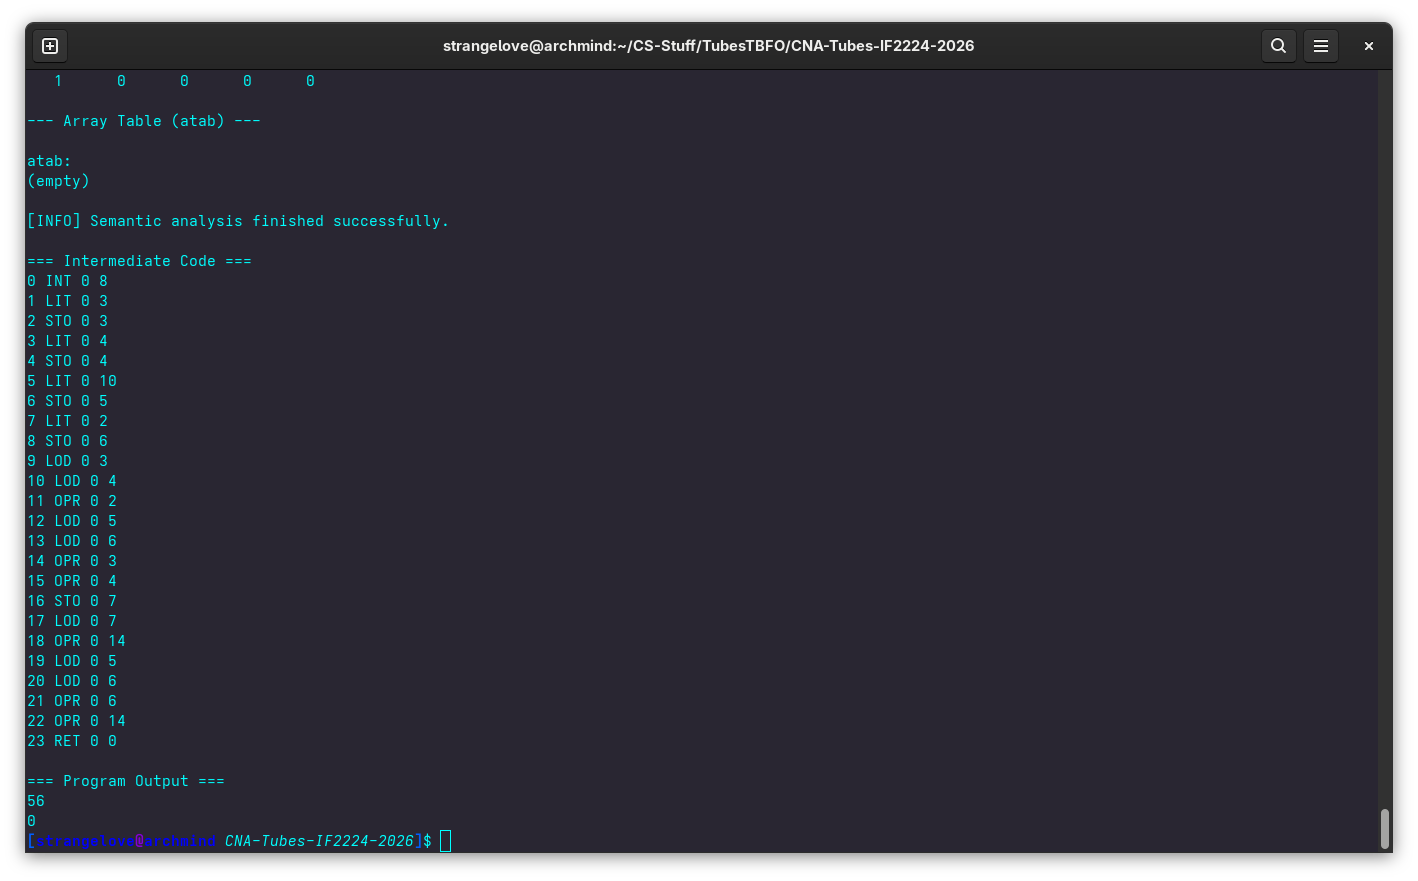
\includegraphics[width=15cm]{gambar/tc3_src_nested_expr.png}
\end{center}

\textbf{Analisis.} $x = (3+4)\times(10-2) = 7 \times 8 = 56$ dan
$c \bmod d = 10 \bmod 2 = 0$. Subekspresi kiri dihitung lebih dulu (OPR 2), lalu
subekspresi kanan (OPR 3), barulah keduanya dikalikan (OPR 4)---membuktikan urutan
evaluasi postorder yang benar tanpa membutuhkan nama \texttt{temporary} eksplisit.

%------------------------------------------------------------------------------
\subsection{Kasus 4 -- Kontrol Alur IF-ELSE dan WHILE}

\textbf{Tujuan.} Menguji translasi percabangan dan perulangan---konvensi
\emph{IF\_FALSE} pada \texttt{JPC}, lompat-mundur \texttt{JMP} pada \texttt{while}.
Kasus ini merupakan contoh kanonik pada spesifikasi.

\begin{minipage}[t]{0.48\textwidth}
\textbf{Masukan} (\texttt{src\_testkeywords.txt}):
\begin{lstlisting}[style=kodeArion, numbers=none]
program TestKeywords;
var
  x, y: integer;
begin
  x := 10;
  if x > 5 then
    y := x * 2
  else
    y := x div 2;
  writeln(y);
  while y > 0 do
  begin
    y := y - 1;
    writeln(y);
  end;
end.
\end{lstlisting}
\end{minipage}\hfill
\begin{minipage}[t]{0.48\textwidth}
\textbf{Intermediate Code:}
\begin{lstlisting}[style=kodeTAC, numbers=none]
1 INT 0 5      16 STO 0 4
2 LIT 0 10     17 LOD 0 4
3 STO 0 3      18 OPR 0 14
4 LOD 0 3      19 LOD 0 4
5 LIT 0 5      20 LIT 0 0
6 OPR 0 11     21 OPR 0 11
7 JPC 0 13     22 JPC 0 30
8 LOD 0 3      23 LOD 0 4
9 LIT 0 2      24 LIT 0 1
10 OPR 0 4     25 OPR 0 3
11 STO 0 4     26 STO 0 4
12 JMP 0 17    27 LOD 0 4
13 LOD 0 3     28 OPR 0 14
14 LIT 0 2     29 JMP 0 19
15 OPR 0 5     30 RET 0 0
\end{lstlisting}
\end{minipage}

\textbf{Keluaran Program:} cabang \texttt{then} terpilih ($x=10>5$) sehingga
$y = 20$, lalu perulangan menghitung mundur hingga 0.
\begin{lstlisting}[style=kodeTAC, numbers=none]
20  19  18  17  16  15  14  13  12  11  10
 9   8   7   6   5   4   3   2   1   0
\end{lstlisting}
\noindent(keluaran sebenarnya satu nilai per baris; ditampilkan dua baris di sini
demi keringkasan).

\begin{center}
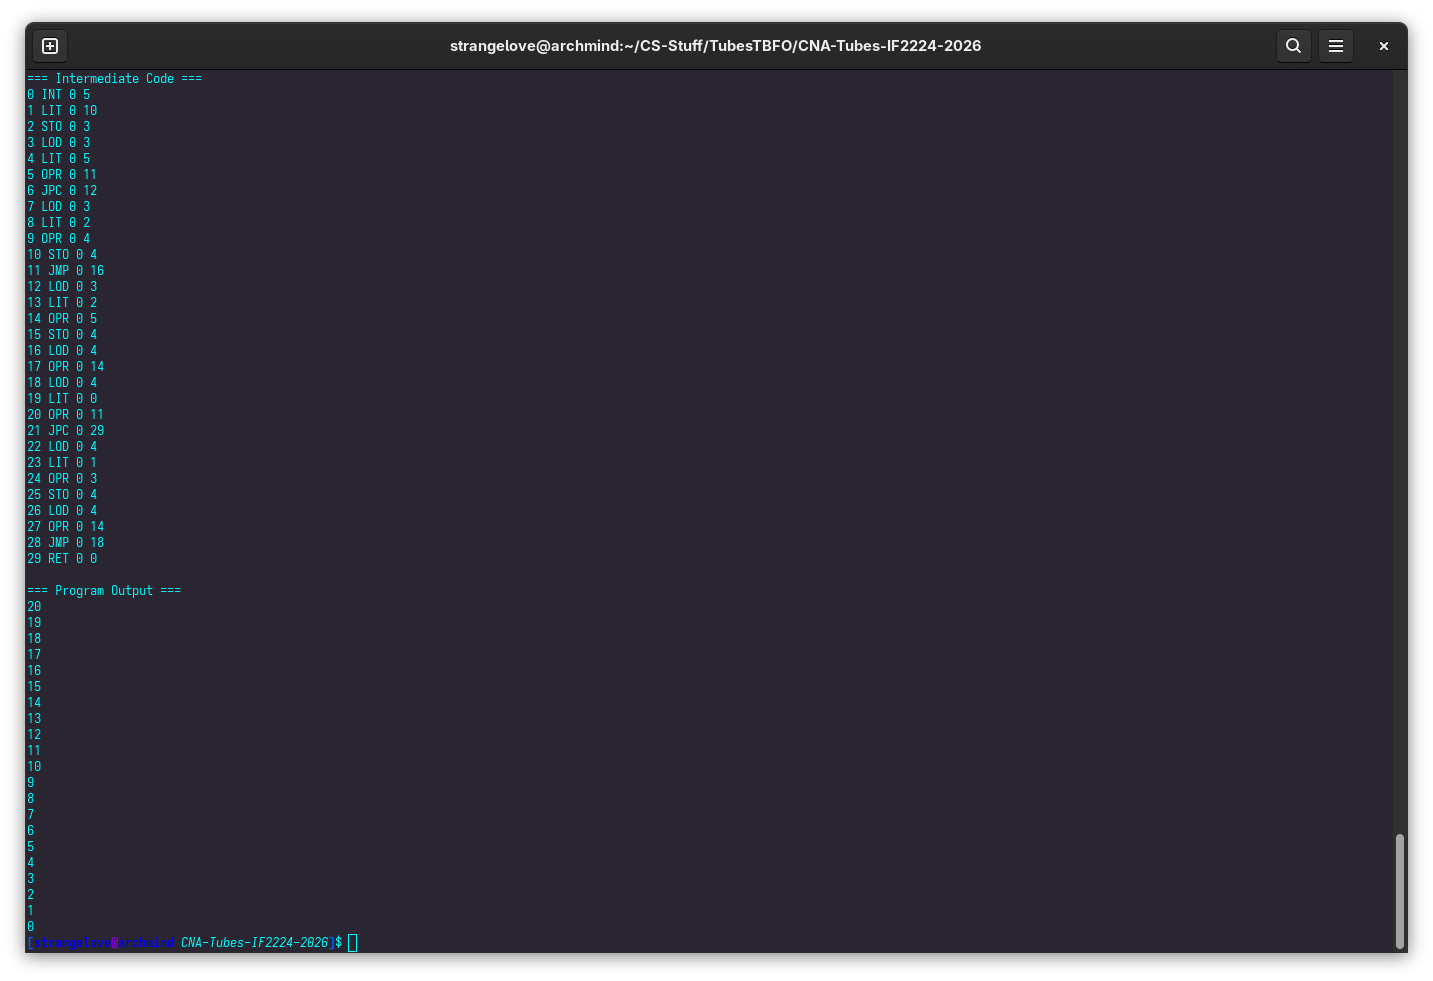
\includegraphics[width=15cm]{gambar/tc4_src_testkeywords.png}
\end{center}

\textbf{Analisis.} Intermediate Code yang dihasilkan identik dengan contoh pada
spesifikasi. \texttt{JPC 0 13} melompati blok \texttt{then} bila kondisi salah,
\texttt{JMP 0 17} melewati blok \texttt{else}, dan \texttt{JMP 0 19} pada
perulangan kembali ke evaluasi kondisi---membuktikan translasi control flow tepat.

%------------------------------------------------------------------------------
\subsection{Kasus 5 -- Penanganan Error: Pembagian dengan Nol}

\textbf{Tujuan.} Memverifikasi bahwa kesalahan runtime tidak membuat program
\emph{crash}, melainkan ditangkap dan dilaporkan secara \emph{graceful}.

\begin{minipage}[t]{0.48\textwidth}
\textbf{Masukan} (\texttt{src\_divzero.txt}):
\begin{lstlisting}[style=kodeArion, numbers=none]
program DivByZero;
var
  a, b: integer;
begin
  a := 10;
  b := 0;
  writeln(a div b);
end.
\end{lstlisting}
\end{minipage}\hfill
\begin{minipage}[t]{0.48\textwidth}
\textbf{Intermediate Code:}
\begin{lstlisting}[style=kodeTAC, numbers=none]
1 INT 0 5
2 LIT 0 10
3 STO 0 3
4 LIT 0 0
5 STO 0 4
6 LOD 0 3
7 LOD 0 4
8 OPR 0 5     ; a div b
9 OPR 0 14
10 RET 0 0
\end{lstlisting}
\end{minipage}

\textbf{Keluaran Program:}
\begin{lstlisting}[style=kodeTAC, numbers=none]
[ERROR] DivisionByZeroError: division by zero !
\end{lstlisting}

\begin{center}
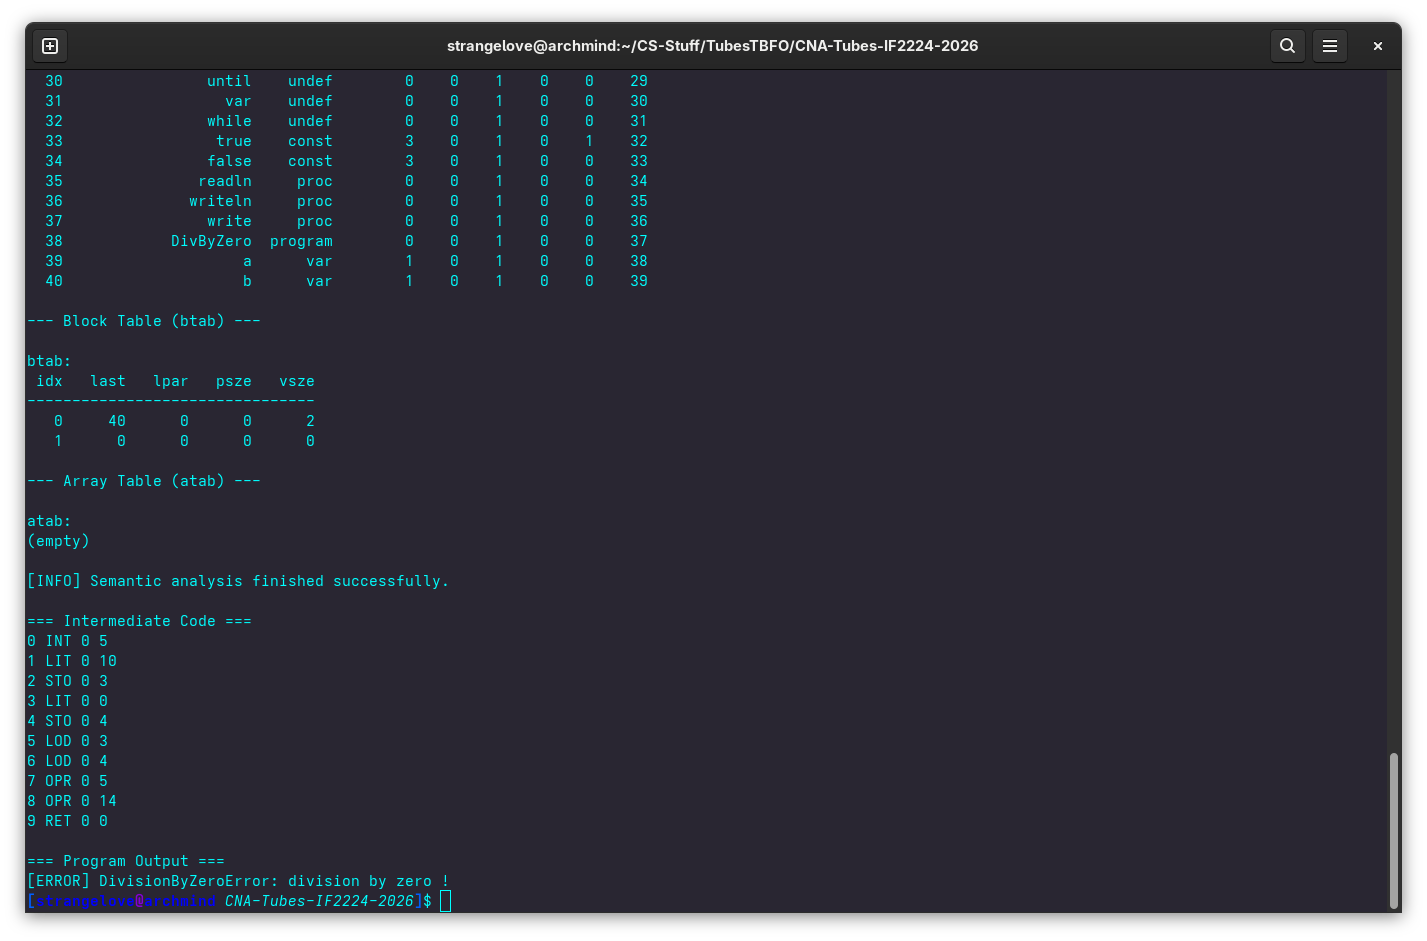
\includegraphics[width=15cm]{gambar/tc5_src_divzero.png}
\end{center}

\textbf{Analisis.} Saat \texttt{DIV} (OPR 5) mendeteksi pembagi bernilai nol,
\texttt{RuntimeErrorHook::divisionByZero()} melempar \texttt{RuntimeError} yang
ditangkap \texttt{Interpreter::run()}. Program berhenti dengan pesan jelas, bukan
\emph{segmentation fault}.

%------------------------------------------------------------------------------
\subsection{Kasus 6 -- Penanganan Error: Numerical Overflow}

\textbf{Tujuan.} Menguji deteksi \emph{integer overflow} pada operasi aritmatika
sebelum nilai sempat membungkus (\emph{wrap-around}).

\begin{minipage}[t]{0.48\textwidth}
\textbf{Masukan} (\texttt{src\_overflow.txt}):
\begin{lstlisting}[style=kodeArion, numbers=none]
program NumericOverflow;
var
  big, hasil: integer;
begin
  big := 4000000000;
  hasil := big * big;
  writeln(hasil);
end.
\end{lstlisting}
\end{minipage}\hfill
\begin{minipage}[t]{0.48\textwidth}
\textbf{Intermediate Code:}
\begin{lstlisting}[style=kodeTAC, numbers=none]
1 INT 0 5
2 LIT 0 4000000000
3 STO 0 3
4 LOD 0 3
5 LOD 0 3
6 OPR 0 4     ; big * big
7 STO 0 4
8 LOD 0 4
9 OPR 0 14
10 RET 0 0
\end{lstlisting}
\end{minipage}

\textbf{Keluaran Program:}
\begin{lstlisting}[style=kodeTAC, numbers=none]
[ERROR] OverflowError: 'MUL' result exceeds the maximum integer value !
\end{lstlisting}

\begin{center}
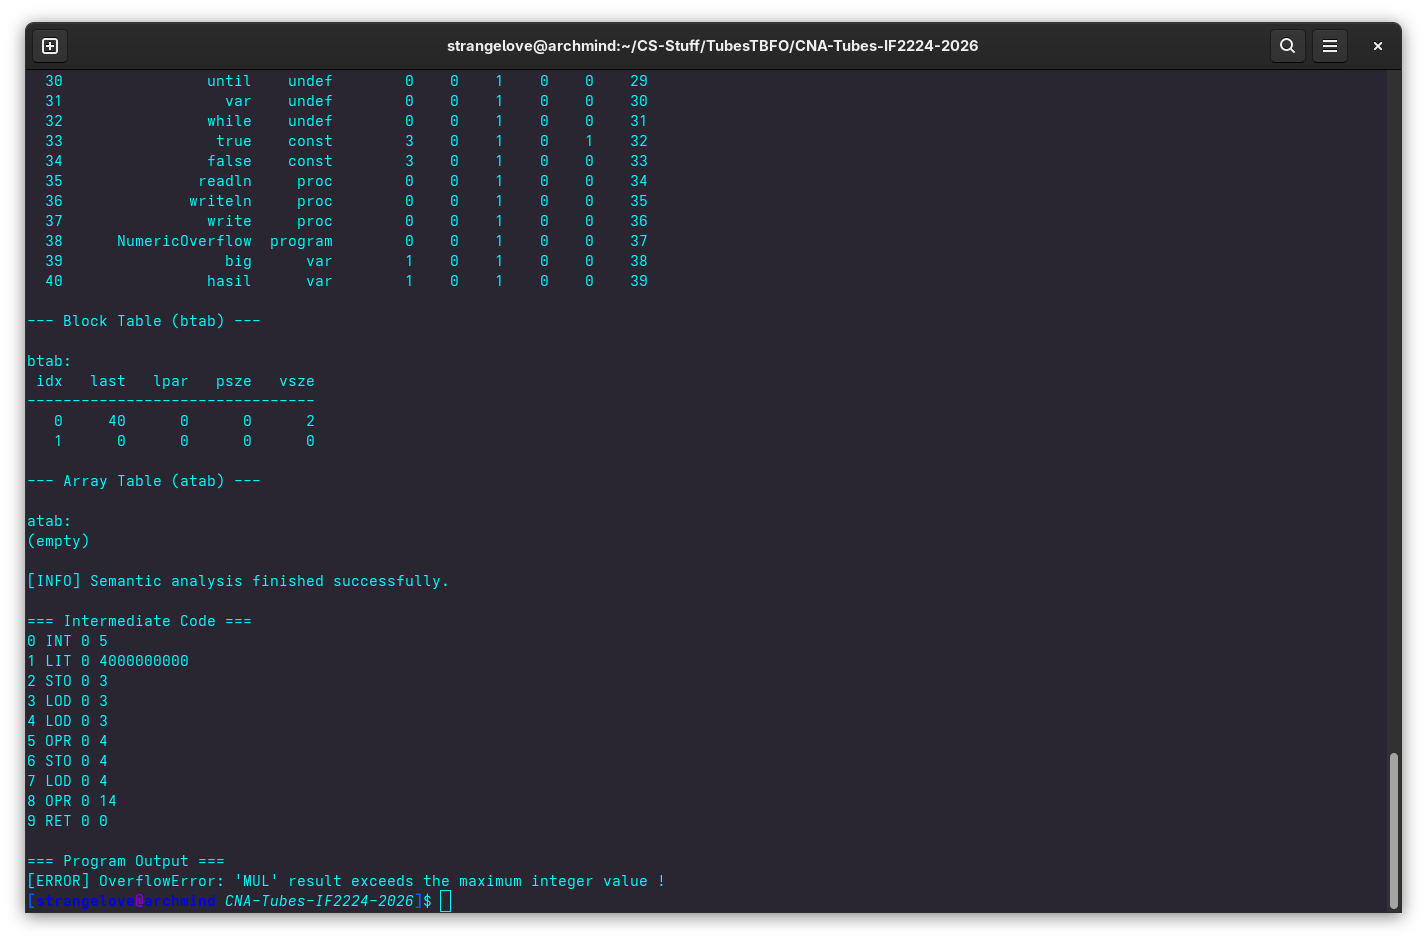
\includegraphics[width=15cm]{gambar/tc6_src_overflow.png}
\end{center}

\textbf{Analisis.} $4{,}000{,}000{,}000^2 = 1.6 \times 10^{19}$ melampaui batas
maksimum integer. \texttt{mulChecked} mendeteksinya melalui
\texttt{\_\_builtin\_mul\_overflow} dan melempar \texttt{OverflowError}, sehingga
hasil yang salah akibat \emph{wrap-around} tidak pernah dicetak.

%------------------------------------------------------------------------------
\subsection{Ringkasan Pengujian}

\begin{table}[H]
\centering
\caption{Ringkasan hasil pengujian Milestone 4.}
\renewcommand{\arraystretch}{1.2}
\begin{tabularx}{\textwidth}{@{}c X l c@{}}
\toprule
\textbf{No} & \textbf{Aspek yang Diuji} & \textbf{Keluaran} & \textbf{Status} \\
\midrule
1 & Penugasan \& cetak literal            & \texttt{10, 99}          & Sesuai \\
2 & Aritmatika \& relasional              & \texttt{10,24,4,TRUE,TRUE} & Sesuai \\
3 & Ekspresi bersarang \& modulus         & \texttt{56, 0}           & Sesuai \\
4 & Control flow IF-ELSE \& WHILE         & \texttt{20\dots0}        & Sesuai \\
5 & Error: pembagian dengan nol           & DivisionByZeroError      & Sesuai \\
6 & Error: numerical overflow             & OverflowError            & Sesuai \\
\bottomrule
\end{tabularx}
\end{table}

Keenam kasus uji memberikan hasil sesuai harapan. Generator menghasilkan
Intermediate Code yang valid (identik dengan contoh spesifikasi pada Kasus 4),
interpreter mengeksekusinya dengan benar, dan mekanisme keamanan runtime berhasil
menangkap kondisi error tanpa menyebabkan program \emph{crash}.
